\section{Common Pipeline Results}

All results from the common pipeline were tested on the validation sets to avoid using the test set too early.

\subsection{Multi-class Classification}

On the mini-MIAS dataset (multi-class classification problem), an accuracy of 50\% was achieved, with a confusion matrix (see Figure~\ref{fig:evaluation-common-CM-norm_basic-model_mini-MIAS-dataset}) indicating that the CNN is confusing cancerous cases together (benign and malignant), but can tell normal cases apart.

\begin{figure}[ht]
\centerline{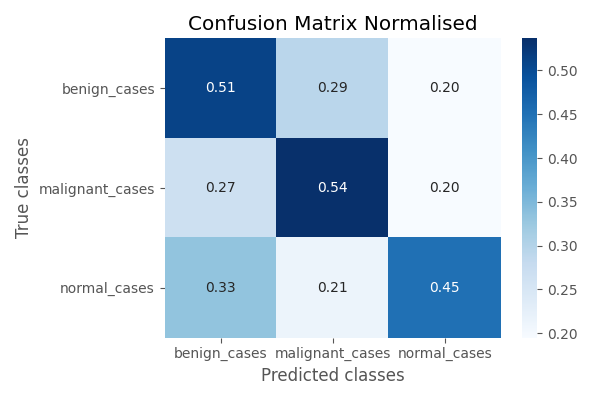
\includegraphics[width=0.8\textwidth]{figures/evaluation/common/CM-norm_basic-model_mini-MIAS-dataset.png}}
\caption{\label{fig:evaluation-common-CM-norm_basic-model_mini-MIAS-dataset}Normalised confusion matrix of the classification results after training on the mini-MIAS dataset.}
\end{figure}

\subsection{Binary Classification}

On the CBIS-DDSM dataset (binary classification problem), an accuracy of 65.36\% was initially achieved. Separating the types of mammograms between calcifications and masses revealed that higher accuracies could be achieved. Indeed, an accuracy of 70.36\% was reached when using only mammograms with masses, and 68.2\%  using only mammograms with calcifications (see Figure~\ref{fig:evaluation-cbisddsm-common-mass-vs-calc}).

\begin{figure}[h]
\centering
\begin{subfigure}{.5\textwidth}
  \centering
  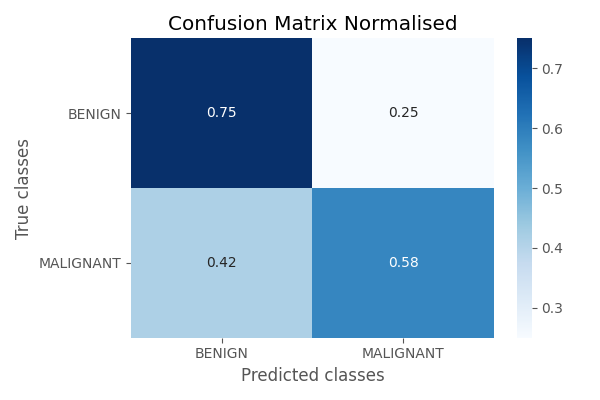
\includegraphics[width=\textwidth]{figures/evaluation/common/CM-norm_basic-model_CBIS-DDSM-dataset-Calc.png}
  \caption{Mammograms with calcifications (70.36\%).}
  \label{fig:evaluation-cbisddsm-common-calc}
\end{subfigure}%
\begin{subfigure}{.5\textwidth}
  \centering
  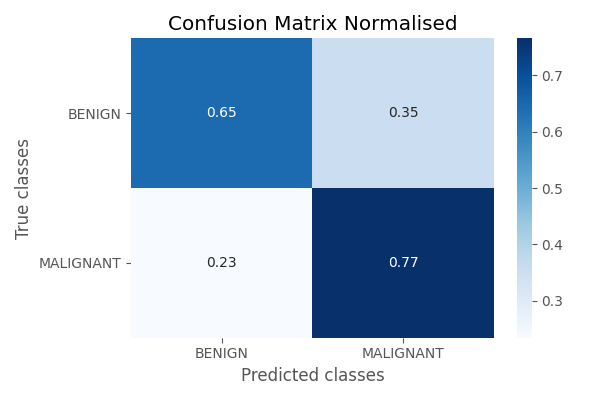
\includegraphics[width=\textwidth]{figures/evaluation/common/CM-norm_basic-model_CBIS-DDSM-dataset-Mass.png}
  \caption{Mammograms with masses (68.2\%).}
  \label{fig:evaluation-cbisddsm-common-mass}
\end{subfigure}
\caption{\label{fig:evaluation-cbisddsm-common-mass-vs-calc}Normalised confusion matrices between mammograms with calcifications and masses on the CBIS-DDSM dataset.}
\end{figure}

Minor optimisation attempts such as adding additional convolutional layers between the pre-trained VGG19 model and the fully connected layers lowered the accuracy to 55.07\%. Adding more convolutional and spooling layers before the VGG19 pre-trained model slightly increased the accuracy from 65.03\% to 65.36\%, but was much slower to train due to the increased number of trainable parameters that originated from the additional layers.

%%%%%%%%%%%%%%%%%%%%%%%%%%%%%%%%%%%%%%%%%%%%%

\section{Individual Optimisation Results}

Using more advanced models than VGG19, which is a sequential CNN, such as InceptionV3, yielded poor results and required much longer training times. Indeed, the evolution of the validation loss visualised in Figure~\ref{fig:evaluation-individual-inceptionv3-poor-training}  confirms that  the InceptionV3 model highly overfits the data, suggested an urgent need for regularisation techniques such as Dropout.\\

\begin{figure}[ht]
\centerline{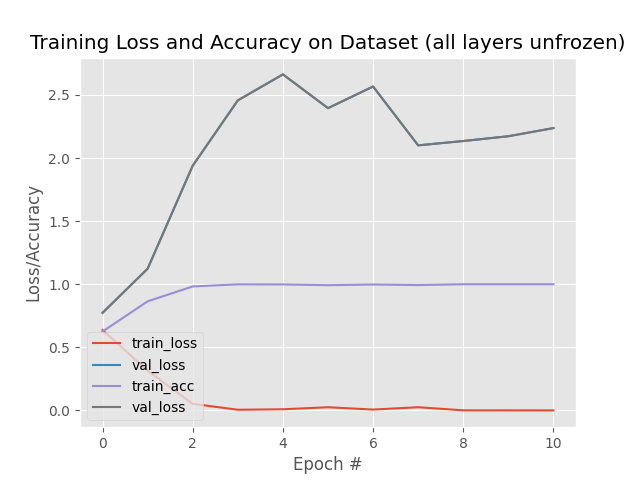
\includegraphics[width=0.8\textwidth]{figures/evaluation/individual/InceptionV3-poor-training.png}}
\caption{\label{fig:evaluation-individual-inceptionv3-poor-training}Evolution of validation loss during training of the InceptionV3 model on the CBIS-DDSM dataset.}
\end{figure}

Potential future comparisons:
\begin{itemize}
    \item Different CNN models (VGG19, ResNet50V2, InceptionV3, Xception)
    \item Using transfer learning (pre-trained model on ImageNet)
    \item Using different types of mammograms (calcifications only, masses only, both)
\end{itemize}

%%%%%%%%

\subsection{Binary mini-MIAS Transfer Learning}

This experiment consisted of expanding upon the concept of transfer learning for the VGG model using weights pre-trained on ImageNet by transfering the weights of a model trained on a binarised mini-MIAS dataset. To binarise the mini-MIAS dataset, the normal cases were dropped altogether, resulting in a very small dataset of 115 abnormal images (64 benign and 51 malignant). The VGG19 model with custom fully connected layers and dropout layers was then trained with the binary mini-MIAS dataset and the final weights were saved.\\

Four different experiments using identical an CNN architecture and random number generator seeds were run to assess the effect of transfer learning from the binarised mini-MIAS dataset to the larger CBIS-DDSM dataset:
\begin{itemize}
    \item Transfer learning of all layer weights (VGG and fully connected layers instantiated with binary mini-MIAS weights);
    \item Transfer learning of fully connected layer weights (fully connected layers instantiated with binary mini-MIAS weights, VGG layers instantiated with ImageNet weights);
    \item Transfer learning of ImageNet weights only (fully connected layers instantiated with random weights, VGG layers instantiated with ImageNet weights);
    \item No transfer learning (VGG and fully connected layers instantiated with random weights).
\end{itemize}

\begin{figure}[ht]
\centerline{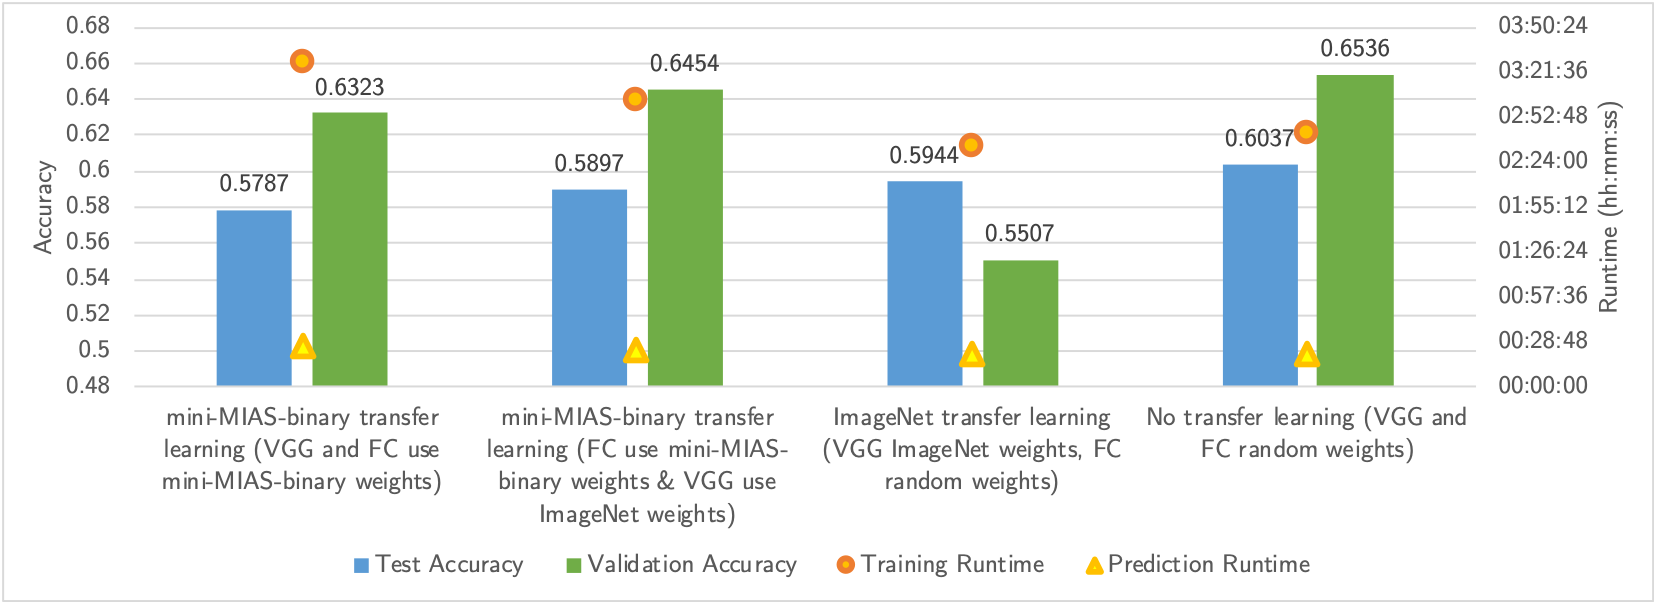
\includegraphics[width=\textwidth]{figures/evaluation/individual/transfer_learning_results.png}}
\caption{\label{fig:evaluation-individual-transfer_learning_results}Results from the transfer learning experiment.}
\end{figure}

A VGG19 model with dense layers replaced by a custom fully connected MLP of size (512, 32, 2) with dropout layers using $p=0.2$ was used, along with an Adam optimiser, initial learning rate of 0.001, batch size of 8 and whole image inputs resized to 512 x 512 pixels.\\

The results clearly indicate that the closer the weight initialisation were to the binary mini-MIAS dataset, the lower the test accuracy was, clearly indicating that the model did not generalise well to CBIS-DDSM mammograms. This could be linked to the advantages of random weight initialisations that give a better chance to the model to explore new combinations of weights rather than immediately converging towards a known solution. Indeed, Figure~\ref{fig:evaluation-individual-TL-training} shows how quickly the loss drops when using binary mini-MIAS weights, whereas the model slowly converges towards a lower loss when using random weight initialisations (no transfer learning).

\begin{figure}[h]
\centering
\begin{subfigure}{.5\textwidth}
  \centering
  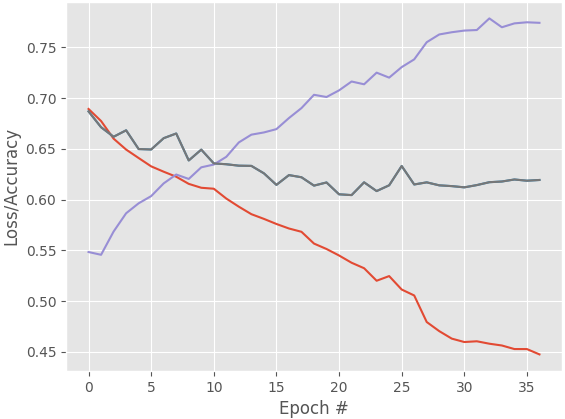
\includegraphics[width=\textwidth]{figures/evaluation/individual/TL-none.png}
  \caption{No transfer learning.}
  \label{fig:evaluation-individual-TL-none}
\end{subfigure}%
\begin{subfigure}{.5\textwidth}
  \centering
  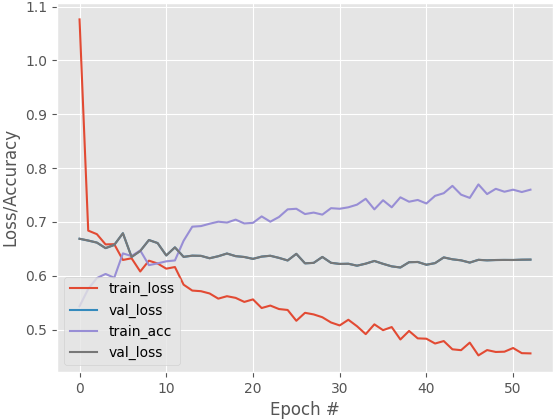
\includegraphics[width=\textwidth]{figures/evaluation/individual/TL-all.png}
  \caption{Binary mini-MIAS on all layers.}
  \label{fig:evaluation-individual-TL-all}
\end{subfigure}
\caption{\label{fig:evaluation-individual-TL-training}Evolution of the training accuracy and the training/validation losses across epochs with a learning rate of 0.001.}
\end{figure}

Additionally, it is worth noting that the training runtimes are similar across all tests, as it is the early stopping conditions (validation loss not decreasing) that dictates the stopping conditions.

\subsection{Mammogram Types}

To assess how the model would react to being fed only specific samples of a single mammogram type, the CBIS-DDSM dataset was separated into only masses samples and only calcifications samples. Three different experiments using identical an CNN architecture were tested:
\begin{itemize}
    \item All types of mammograms (masses + calcifications);
    \item Mass mammograms only;
    \item Calcification mammograms only.
\end{itemize}

\begin{figure}[ht]
\centerline{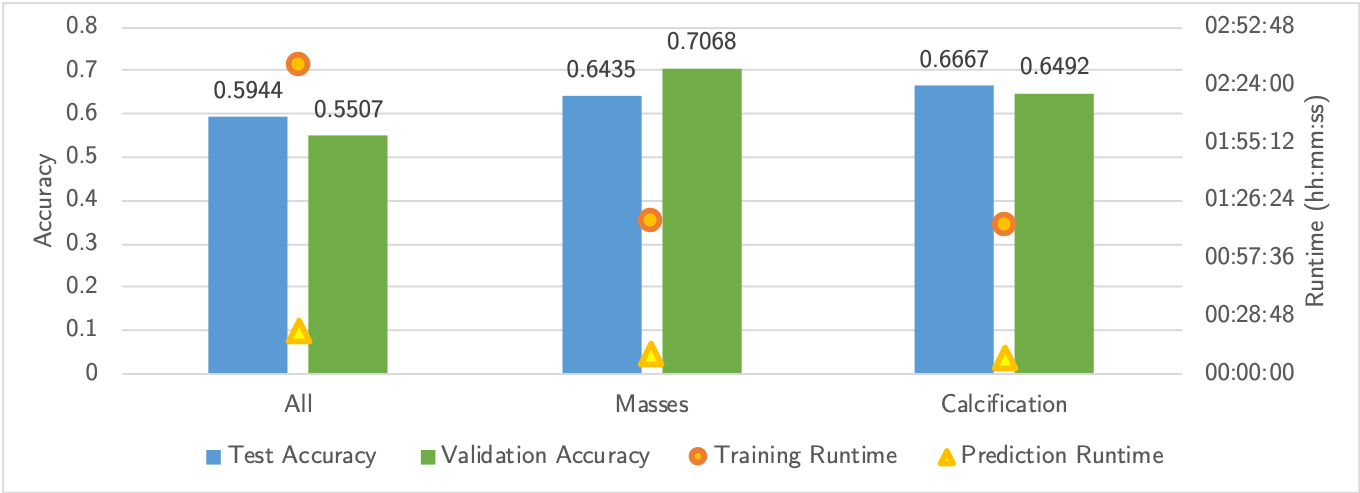
\includegraphics[width=\textwidth]{figures/evaluation/individual/mammogram_types_results.png}}
\caption{\label{fig:evaluation-individual-mammogram_types_results}Results from the different mammogram types experiment.}
\end{figure}

These results show that the model learns the data much better when masses and calcifications are separated, reaching 64.35\% and 66.67\% accuracy respectively on the test set, but only managing 59.44\% when using the full CBIS-DDSM dataset. Indeed, the normalised confusion matrix indicates that all instances are classified as ``benign'' using the full dataset containing both types, which could indicate that the model gets confused when dealing with multiple views.